
\section{Instrumentering}
%Måleteknikk

\begin{center}
\begin{longtable}{ | m{2cm} | m{7cm} | } 
\hline
\multicolumn{2}{|c|}{Definisjoner} \\
\hline
Begrep	& Beskrivelse \\ 
\hline
\hline
	Avvik&Forskjellen mellom den målte verdien og ønsket verdi (skalverdi) i ei reguleringssløyfe\\
	\hline
	Dødgang (dødsone)&For prosessinstrumenter er dødgang det området som et inngangssignal kanforandres innenfor, uten at det vises noen forandring i utgangssignalet. Med forandring menes her reversering av retningen på inngangssignalet\\
	\hline
	Forsterkning&Forholdet mellom forandring i inngangsverdien i forhold til den utgangsverdien som var årsak til forandringen\\
	\hline
	Hysterese&Samme måleverdi kan gi ulike utsignaler fra måleomformeren ved samme verdi, Hysterese oppstår når måleverdien veksler mellom å være stigende eller fallende.\\
	\hline
	Kalibrering&Sjekk av at måleinstrumentets verdier stemmer med et intrument med høyere nøyaktihet. Noen intrumenter kan justeres inn om de ikke stemmer overens.\\ 
	\hline
	Lesbarhet&Den minste inndeling på skalaen på et instrument.\\
	\hline
	Måleomfang&Differansen mellom øvre og nedre målegrense\\
	\hline
	Målegrense&URV: høyeste verdi som instrumentet kan vise. LRV: laveste verdi som instrumentet kan vise. \\
	\hline
	Målegrense&Den fulle skalaen for en måling, indikering eller avlesning. Eksempelvis -50 til 150°C\\
	\hline
	Nullpunktfeil&En forskyving av nede målegrense\\
	\hline
	Nøyaktighet& Forskjell mellom avlest og virkelig verdi for en målt variabel.\\
	\hline

	Reproduser- barhet& Evnen til å reprodusere samme resultat fra en rekke uavhengige målinger av den samme verdien selv om målingen utføres av forskjellige personer, på forskjellige steder og under ulike klimatiske forhold.\\
	\hline
	Repeterbarhet&Samsvar mellom en rekke på hverandre følgende målinger av utgangsverdi for den samme inngangsverdien. Målingene foretas under samme klimatiske forhold, av samme person og med korte intervaller.\\
	\hline
	Ulinearitet&En type feil der inngangsverdiene til et instrument ikke forholder seg til den ideelle rettlinjede sammenhengen mellom inngangs- og utgangs-verdiene (referansekarakteristikken).\\
	\hline

Regulator & En enhet som har til oppgave å påvirke prosessen slik at den oppnår en ønsket tilstand (f.eks. et ønsket nivå eller en ønsket temperatur).\\
	\hline
Prosess & Det anlegget eller systemet som inngår i reguleringen.\\
	\hline
Prosessvariabel & Den fysiske størrelsen i prosessen som skal reguleres (nivå, trykk, temperatur etc.)\\
	\hline
ProsessVerdi PV & Den verdien prosessvariabelen til enhver tid har.\\
	\hline
Settpunkt SP & Den verdien vi ønsker at prosessvariabelen skal ha.\\
	\hline
Manipulerende Variabel MV & Signalet som styrer pådragsorganet\\
	\hline
Forsyning & \\
	\hline
Pådrag & Det som er ment å variere prosessvariabelen. F.eks. væske inn i en nivåtank. \\
	\hline
Belastning & Det som tas ut av prosessen ved konstant PV. Vil ha samme verdi som pådraget. \\
	\hline
Forstyrrelse & Forandringer som påvirker verdien til prosessvariabelen. \\
	\hline
Avviket e & Forskjellen mellom PV og SP (Direkte virkning PV-SP, Reverserende virkning SP-PV)\\
	\hline
Pådragsorgan & Den komponenten som styrer pådraget (f.eks. motoren i bilen som påvirker hastigheten, eller ventilen som påvirker nivået i tanken).\\
	\hline
Forstillingsenhet & I vårt eksempel med regulering av bilens hastighet, er forstillingsenheten forgasseren. Motoren er pådragsorganet i reguleringssløyfen.\\
	\hline
Auto og Manuell modus (Lukket& eller åpensløyfe). Om pådraget styres av regulatoren eller en manuell innstilt verdi. \\
	\hline
LRV og URV& ( Lover Range Value og Upper Range value, Laveste og høyeste verdi målesignalet kan ha.)\\

	\hline


\end{longtable}
\end{center}
\vskip 5pt
\hrule

\vskip 5pt
\subsection{Kalibrering}
Kalibrering vil si at en sjekker at måleinstrumentets verdier stemmer med et intrument med høyere nøyaktihet. Noen intrumenter kan justeres inn om verdien ikke er innenfor kravet. Etter denne justeringen kan en da gjøre en ny sjekk av måleinstrumentets verdier. 

\vskip 5pt 
$$\includegraphics[width=1\textwidth]{calibrate31.eps}$$

\filbreak

$$\includegraphics[width=1\textwidth]{calibrate26.eps}$$
$$\includegraphics[width=1\textwidth]{calibrate32.eps}$$
\filbreak
\vskip 5pt 

I 3AUA bruker vi 5-punkts opp/ned sjekk når vi kalibrerer instrumenter. 

\vfil \eject
\large
\begin{center}
\begin{tabular}{ | m{2cm} | m{2cm} |m{2cm} |m{2cm} |m{2cm} |} 
\hline
	\multicolumn{5}{|c|}{\textbf{\cellcolor[HTML]{D5D5D5}Kalibreringsskjema for 3AUA Gand}} \\
\hline
\hline
\hline
	\multicolumn{5}{|c|}{\textbf{\cellcolor[HTML]{D5D5D5}Instrument informasjon}}\\
\hline
	System tag&	\multicolumn{2}{l|}{Produsent}&\multicolumn{2}{l|}{Modell}\\
\hline
&	\multicolumn{2}{l|}{}&\multicolumn{2}{l|}{}\\
\hline
	C.Intervall&\multicolumn{2}{l|}{Serienr.}&LRV&URV\\
\hline
	&	\multicolumn{2}{l|}{}&&\\
\hline
	\multicolumn{5}{|c|}{\textbf{\cellcolor[HTML]{D5D5D5}Feil \%} }\\
\hline
	Største feil&Zero&Span&Liearitet&Hysterese\\
\hline
	&&&&\\
\hline
	\multicolumn{5}{|c|}{\cellcolor[HTML]{D5D5D5}\textbf{As Found resultater}}\\
\hline
	Test punkt	&Inngang&Utgang&Utgangsfeil&Utg.feil \%\\
\hline
1&&&&\\
\hline
2&&&&\\
\hline
3&&&&\\
\hline
4&&&&\\
\hline
5&&&&\\
\hline
4&&&&\\
\hline
3&&&&\\
\hline
2&&&&\\
\hline
1&&&&\\
\hline
	\multicolumn{5}{|c|}{\cellcolor[HTML]{D5D5D5}\textbf{As left resultater}}\\
\hline
	Test punkt	&Inngang&Utgang&Utgangsfeil&Utg.feil \%\\
\hline
1&&&&\\
\hline
2&&&&\\
\hline
3&&&&\\
\hline
4&&&&\\
\hline
5&&&&\\
\hline
4&&&&\\
\hline
3&&&&\\
\hline
2&&&&\\
\hline
1&&&&\\
\hline
	\multicolumn{5}{|c|}{\textbf{\cellcolor[HTML]{D5D5D5}Underskrifter}}\\
\hline
	\multicolumn{5}{|l|}{\textbf{Dato:}}\\
\hline
	\multicolumn{3}{|l|}{\textbf{Elev}}&\multicolumn{2}{l|}{\textbf{Lærer}}\\
\hline
	\multicolumn{3}{|c|}{}&\multicolumn{2}{c|}{}\\
\hline
\end{tabular}
\end{center}
\normalsize
\vfil \eject

\subsubsection{Generell sløyfetestprosedyre}
\begin{enumerate}
\item Sjekk at P\&ID tegning for denne sløyfa stemmer med Virkeligheten.
\item Oppdater P\&ID, evt. merk med \textquotedblright AS BUILT\textquotedblright ,
navn og dato
\item Sjekk at looptegningen for denne sløyfa stemmer med virkeligheten.
\item Oppdater looptegning, evt. merk med \textquotedblright AS BUILT\textquotedblright \textquotedblright ,
navn og dato.
\item Sjekk at datasheet for instrumentene i sløyfa stemmer.
\item Sjekk installasjon, (fyll ut \textquotedblright Punchlist\textquotedblright{}
for feil og mangler.)
\item Koble til HART communikator, sjekk at TAG nummer er lagt inn, sjekk
at LRV og URV stemmer med datasheet.
\item Sjekk at det er kalibreringssertifikat for alle instrumentene i sløyfa,
hvis ikke må instrumentene kalibreres og kalibreringssertifikat fylles
ut.
\item Simulering/testing
\begin{enumerate}
\item Ved simulering av trykk, sørg for å drenere/blåse ut evt. væske fra
transmitteren. Koble simulator for inngangssignal til transmitteren
(händpumpe/manometer) og mA meter på utgangen. Kjør 5 pkt. sjekk,
les av og noter resultat på alle instrumentene i sløyfa (kan kombineres
med pkt. 8) Ved tilbakekobling sørg for å lufte transmitteren, særlig
ved lave trykk.
\item Ved simulering av temperatur, koble simulator for inngangssignal til
transmitteren. (temperaturkalibrator eller dekadeboks etc. og mA meter
på utgangen. Kjør Spkt. sjekk, les av og noter resultat på alle instrumentene
i sløyfa (kan kombineres med pkt. 8). Koble tilbake elementet og sjekk
at transmitteren viser romtemperatur.
\end{enumerate}
\item Sjekk alarmsetpunkter og funksjon.
\item Fyll ut looptestsertifikat
\end{enumerate}





\vfil \eject
\subsubsection{Skallering}
$$\includegraphics{current63.eps}$$

Ut fra denne representasjonen kan vi sette opp følgende formel for konvertering mellom signaler. 
$$		\frac{y-y_{start}}{y_{range}}=\frac{x-x_{start}}{x_{range}}$$

$$\includegraphics{current59.eps}$$
\vfil \eject











